% TODO introduire l'application, les fonctionnalités et les types d'user brièvement

\chapter{Analyse des besoins}
% Partie dans laquelle on explique les features / requirements attendues
% On y trouve sans doute :

\epigraph{<< Les choses paraissent simples jusqu'à ce qu'on commence à les analyser >>}{Audrey Niffenegger}

La phase d'analyse est dans la vie d'un projet l'une des phases les plus critiques car celle-ci formalise les besoins des clients sous tous ses aspects afin que toutes les parties (dont les développeurs) puissent se mettre d'accord. Pour pallier les nombreuses difficultés inhérentes au contexte, plusieurs méthodes reconnues existent (notamment \Gls{QQOQCCP} et UML). \\

La principale fonctionnalité attendue de l'application web est la recherche de \glspl{fiche} sur base d'une combinaison de critères divers et variés (dont notamment des \glspl{tag}) pourrait sembler à première vue simple mais il n'en est rien. En effet, la question sous-jacente est le problème du référencement de ressources informatiques. Contrairement à d'autres domaines (par exemple la littérature), il n'existe pas de consensus sur au moins une manière d'organiser les informations d'une ressource informatique.

\section{Analyse fonctionnelle}
\label{section:analyseFonctionnelle}

\subsection*{Séparation des tâches}

Comme expliqué par les Echos\cite{SOD}, la séparation des tâches est "un concept qui requière différents acteurs possédant des rôles et responsabilités différents pour la réalisation d’un ensemble de tâches dont l’exécution par un unique acteur pourrait potentiellement conduire à des fraudes ou des erreurs". \\


En effet, ce catalogue qui repose sur la collaboration d'acteurs variés nécessite un certain nombre de garde-fous afin de maintenir un outil qui dispose de ressources aussi bien de manière qualitative que quantitative. Notre analyse nous a permis d'isoler 4 types d'utilisateurs qui disposent de privilèges de manière incrémentale (en plus de disposer de leurs privilèges propres, chacun hérite aussi de ceux du précédent de la présente liste) :

\begin{itemize}
    \item Visiteur : Il s'agit d'un utilisateur non inscrit à notre plate-forme. Il ne peut rechercher et consulter que les \glspl{fiche} de ressources validés par un administrateur.
    \item Utilisateur : Il s'agit d'un utilisateur  inscrit à notre plate-forme. Celui-ci peut proposer des nouvelles ressources ainsi que de maintenir les \glspl{fiche} dont il est le créateur.
    \item Administrateur : Celui-ci crée/modifie des ressources de toute nature (\glspl{fiche} proposées par les utilisateurs, \glspl{tag} et \glspl{tagCat}), en plus de classifier les \glspl{fiche}.
    \item Super Administrateur : Celui-ci dispose du droit de supprimer de manière définitive les différentes ressources de notre plate-forme.
\end{itemize}

\subsection*{Fonctionnalités}

\subsubsection*{Tout visiteur peut : }

\begin{itemize}
    \item Se connecter à l'application via une adresse mail et un mot de passe
    \item S'inscrire à l'application
    \item Rechercher des \glspl{fiche} dans l'application. La recherche se porte sur une combinaison libre des critères suivants : 
    \begin{itemize}
        \item Rechercher dans le titre des \glspl{fiche}
        \item Rechercher dans les \glspl{tag} des \glspl{fiche} ( cf TODO : Ce point sera expliqué en détail au point x.z.y )
        \item Filtrer les \glspl{fiche} par leurs identifiants
        \item Filtrer les \glspl{fiche} par leurs créateurs
        \item Filtrer les \glspl{fiche} par leurs états
        \item Filtrer les \glspl{fiche} sur base d'un certain seuil sur le résultat moyen accordé par les utilisateurs
    \end{itemize}
    Il est également possible d'y associer les fonctionnalités suivantes :
    \begin{itemize}
        \item Ordonner les \glspl{fiche} avec une libre combinaison des paramètres suivants (en précisant pour chacun l'ordre du tri : ascendant / descendant) :
        \begin{itemize}
            \item le résultat moyen des votants pour une \gls{fiche}
            \item le nombre de votants pour une \gls{fiche}
            \item la date de la dernière modification de la \gls{fiche}
            \item le titre de la \gls{fiche}
            \item l'état de la \gls{fiche}
            \item l'identifiant de la \gls{fiche}
        \end{itemize}
        \item Choisir quelles propriétés des \glspl{fiche} inclure dans le résultat
    \end{itemize}
    \item Consulter une \gls{fiche}
    \item Consulter les \glspl{tag} et \glspl{tagCat} existants ( avec si demandé, des statistiques d'utilisation de ceux ci )
    \item Télécharger la source d'une \gls{fiche} 
\end{itemize}

\subsubsection*{Tout utilisateur peut : }
\begin{itemize}
    \item Consulter / Modifier ses informations personnelles
    \item Mettre en ligne une \gls{fiche}  (avec éventuellement un fichier )
    \item Modifier les informations d'une \gls{fiche}  l'appartenant
    \item Changer l'état d'une \gls{fiche}  l'appartenant ( des restrictions existent pour éviter des dérives )
    \item Proposer un nouveau ou plusieurs mot(s) clé(s)
    \item Évaluer une \gls{fiche}  
    \item \Gls{crud} des recherches favorites
\end{itemize}

\subsubsection*{Tout administrateur peut : }
\begin{itemize}
    \item Exporter des \glspl{fiche} au format JSON
    \item Importer plusieurs \glspl{fiche} sur base d'un fichier JSON.
        Cette fonctionnalité comprend les fonctionnalités sous jacentes suivantes :
        \begin{itemize}
            \item Ajouter éventuellement un état spécifique pour chacune des \glspl{fiche} à importer
            \item Créer automatiquement les \glspl{tag} non existants dans le système (avec éventuellement un état de départ)
            \item Créer automatiquement les \glspl{tagCat} non existantes dans le système
            \item Associer les \glspl{tag} à leurs \glspl{fiche} respectives. 
        \end{itemize}
    \item Proposer un nouveau ou plusieurs mot(s) clé(s) (avec éventuellement un état spécifique pour chacun)
    \item Modifier un \gls{tag} 
    \item Modifier une \gls{tagCat} 
    \item Changer l'état d'un ou plusieurs mot(s) clé(s)
    \item Modifier les informations d'une \gls{fiche} 
    \item Changer l'état d'une \gls{fiche} ( aucune restriction)
    \item Créer ou trouver des \glspl{tagCat}
    \item Lister tous les utilisateurs de l'application ( sans distinction )
\end{itemize}

\subsubsection*{Tout super administrateur peut : }
\begin{itemize}
    \item Supprimer des \glspl{fiche} / \glspl{tag} / \glspl{tagCat}
    \item Modifier le type d'un utilisateur
\end{itemize}
\pagebreak
\subsection*{État d'une \gls{fiche}}

Au cours de notre analyse des processus de partage/modération de ressources informatiques, nous avons été confrontés à de nombreuses lacunes dans des systèmes similaires dont notamment :
\begin{itemize}
    \item Une manière très simplifiée de considérer les \glspl{fiche} : il n'y a pas de nuance claire pour différencier la situation d'une \gls{fiche} par rapport à une autre. Pour l'illustrer, prenons l'exemple d'une \gls{fiche} qui est en cours de rédaction (et donc n'est pas encore prête à être publique) : bien souvent, cette information est absente.
    \item Le manque d'évolutivité technique dans la gestion des \glspl{fiche}, que nous pouvons sans doute imputer à une analyse très restrictive. Conséquence du point précédent, cette lacune rend difficile l'ajout de nouvelles fonctionnalités telles que l'archivage numérique de ces ressources. 
\end{itemize}

C'est ainsi que nous avons décidé d'associer un état à chaque \gls{fiche}, permettant ainsi de distinguer la situation de chacune au cours de ses processus. Le diagramme UML à états ci-dessous représente ces états et les principales transitions entre états (pour ne pas surcharger celui-ci) :

% width=\textwidth,height=\textheight,keepaspectratio
\begin{figure}[H]
    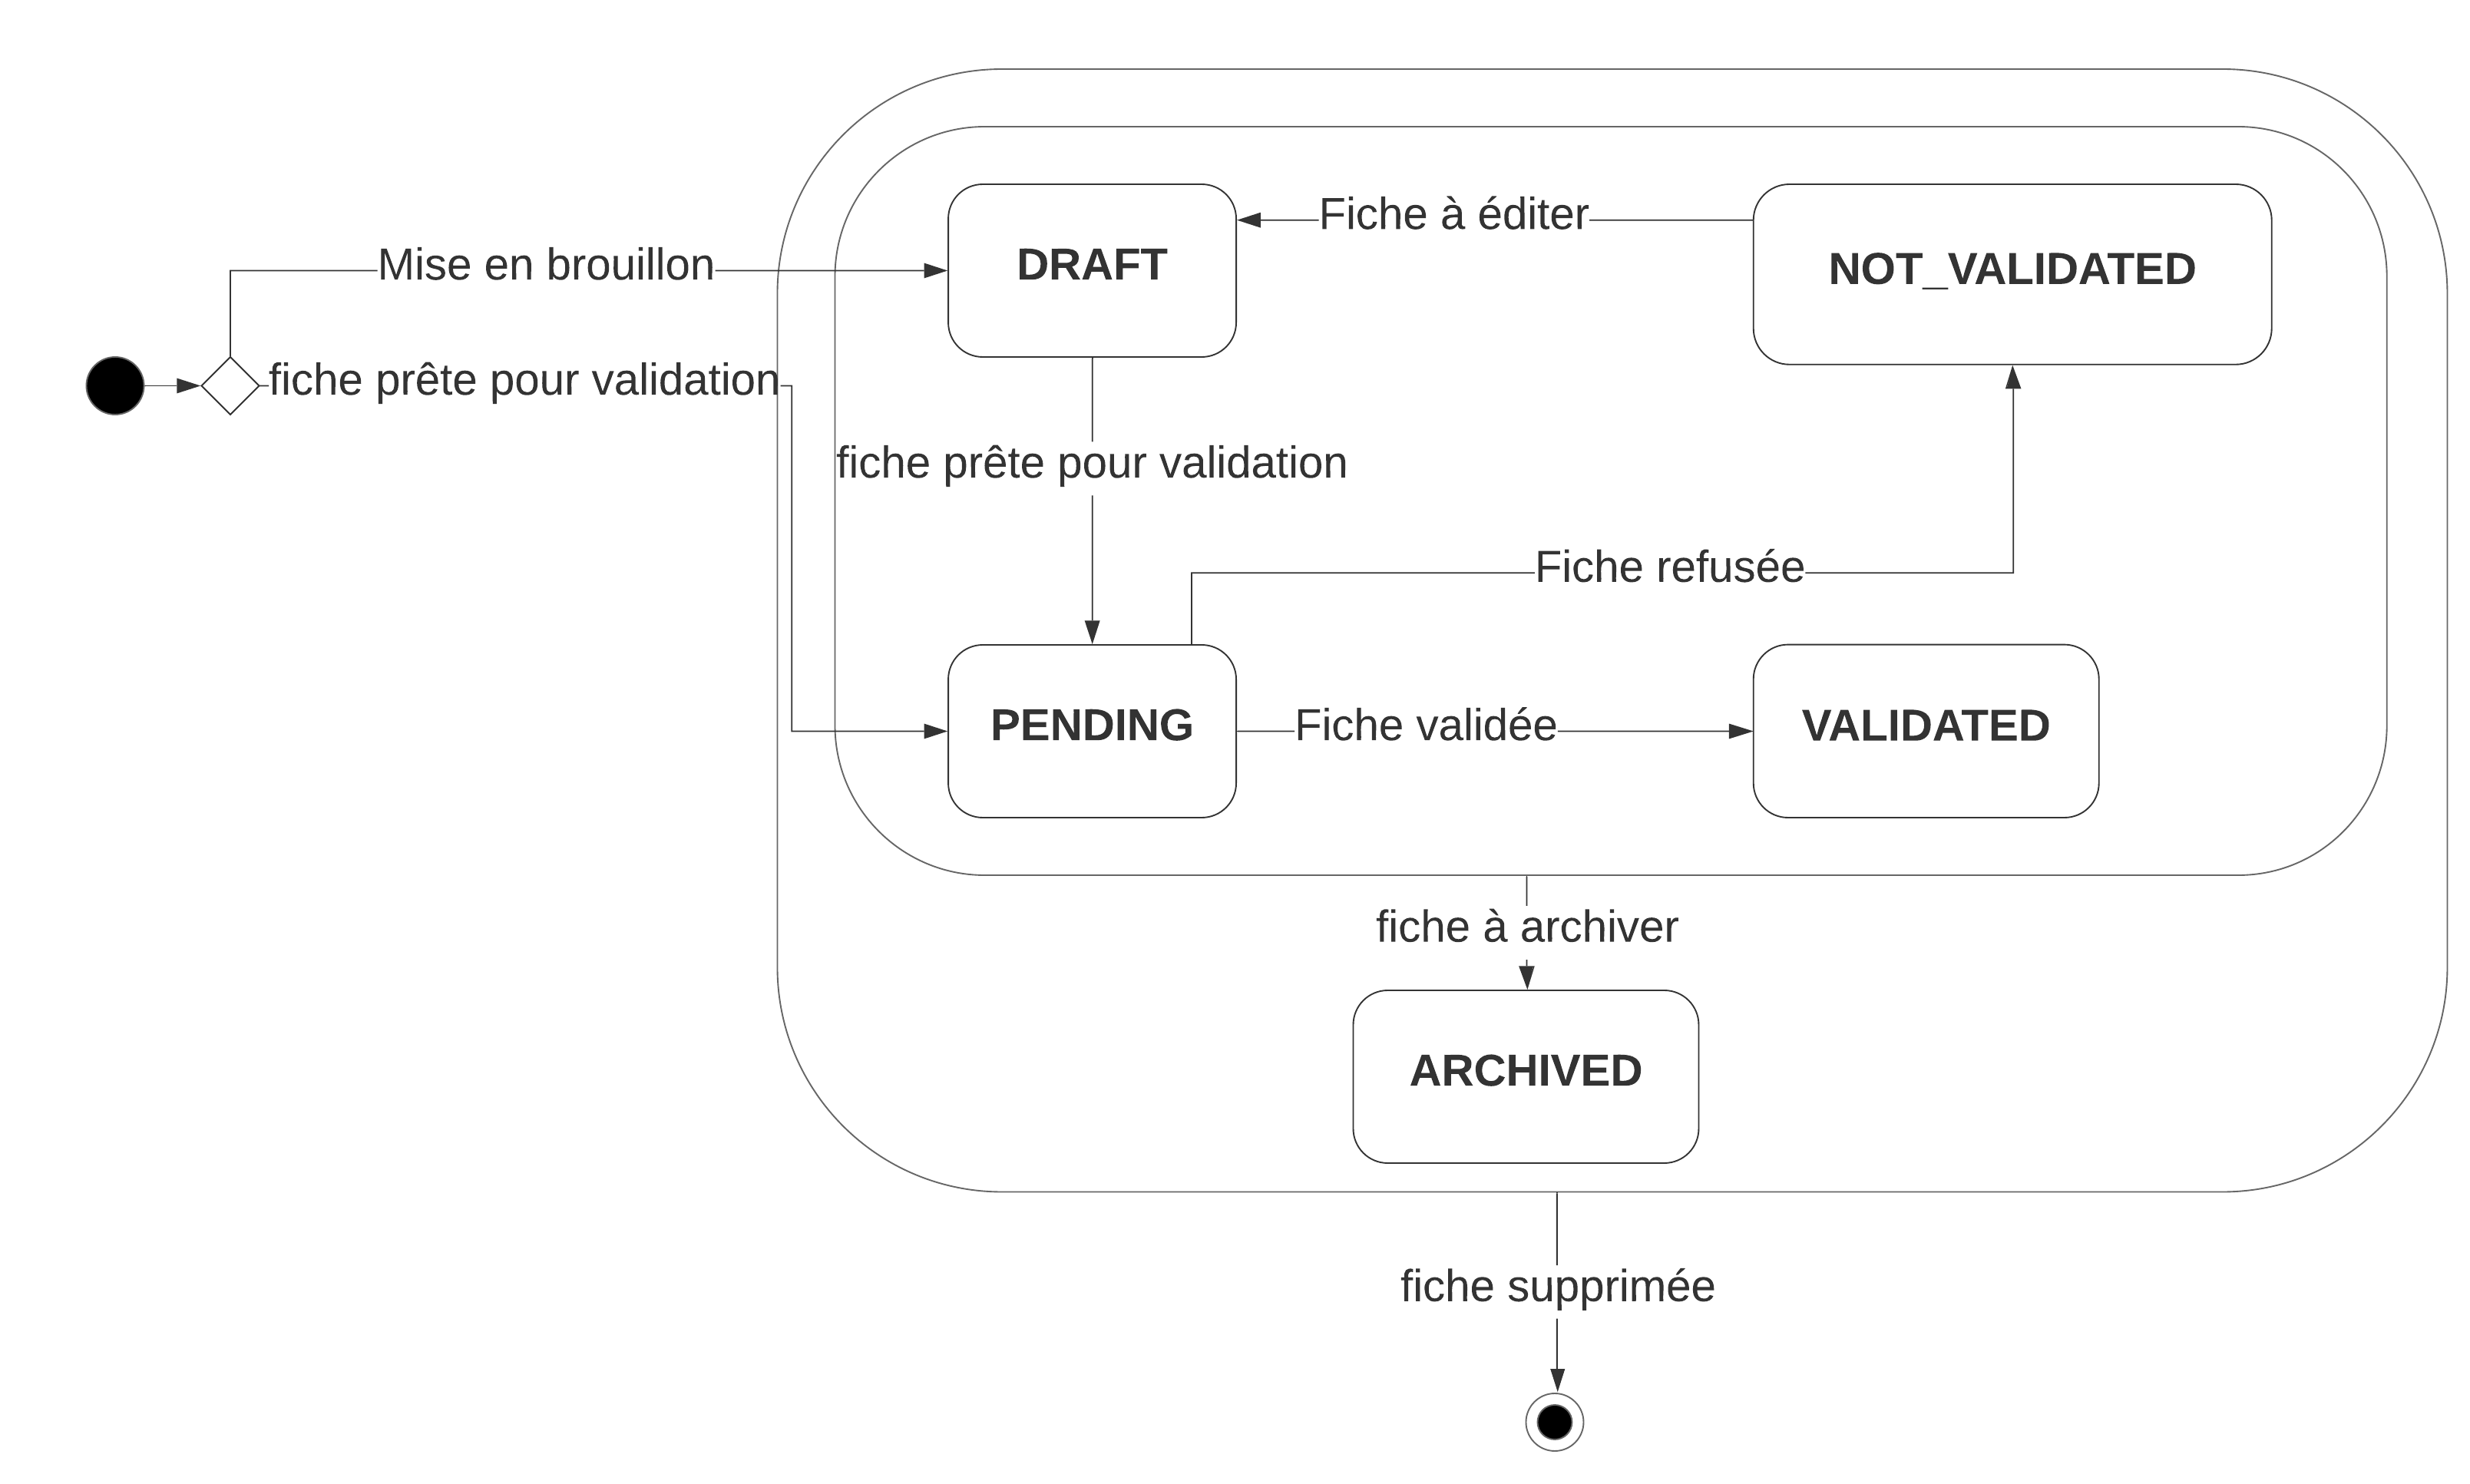
\includegraphics[width=\textwidth,height=\textheight,keepaspectratio]{images/StateFiches.png}
    \centering
    \caption{Diagramme UML à états pour l'état d'une \gls{fiche}}
    \label{pic:stateDiagramForFiches}
\end{figure}

\subsection*{État d'un \gls{tag}}

Une des questions annexes au sujet des \glspl{fiche} est la gestion des \glspl{tag}. En effet, les \glspl{tag} étant des éléments indispensables d'une \gls{fiche} de qualité pour un meilleur référencement, il convient d'établir une stratégie précise pour exploiter au mieux ceux-ci. \\

Durant notre analyse, nous avons pu constater deux écoles de pensée bien distinctes (comparable à ce qui existe en économie) : 
\begin{itemize}
    \item laissez-faire : Il s'agit de donner une liberté totale en matière de marquage (en utilisant aussi bien des \glspl{tag} existants que non). Bien que cette approche a le mérite de faire émerger de nouveaux \glspl{tag} par les contributions d'utilisateurs, cela restreint les possibilités de modération.
    \item l'interventionnisme : Il s'agit de restreindre le choix en matière de marquage (exclusivement des \glspl{tag} existants). Bien que cette approche rend la modération facile, cela restreint les possibilités de s'adapter à une réalité changeante.
\end{itemize}

Nous avons remarqué qu'aucune de ces deux possibilités ne se distinguait suffisamment de l'autre pour répondre de manière optimale à la problématique.
C'est pourquoi nous avons fait le choix d'une 3e voie, qui se situe donc entre ces 2 manières de penser. Tout comme les \glspl{fiche}, il s'agit d'associer un état à chaque \gls{tag} pour distinguer sa situation propre. Le diagramme UML à états ci-dessous représente ces états et les principales transitions entre états (pour ne pas surcharger celui-ci) :

% width=\textwidth,height=\textheight,keepaspectratio
\begin{figure}[H]
    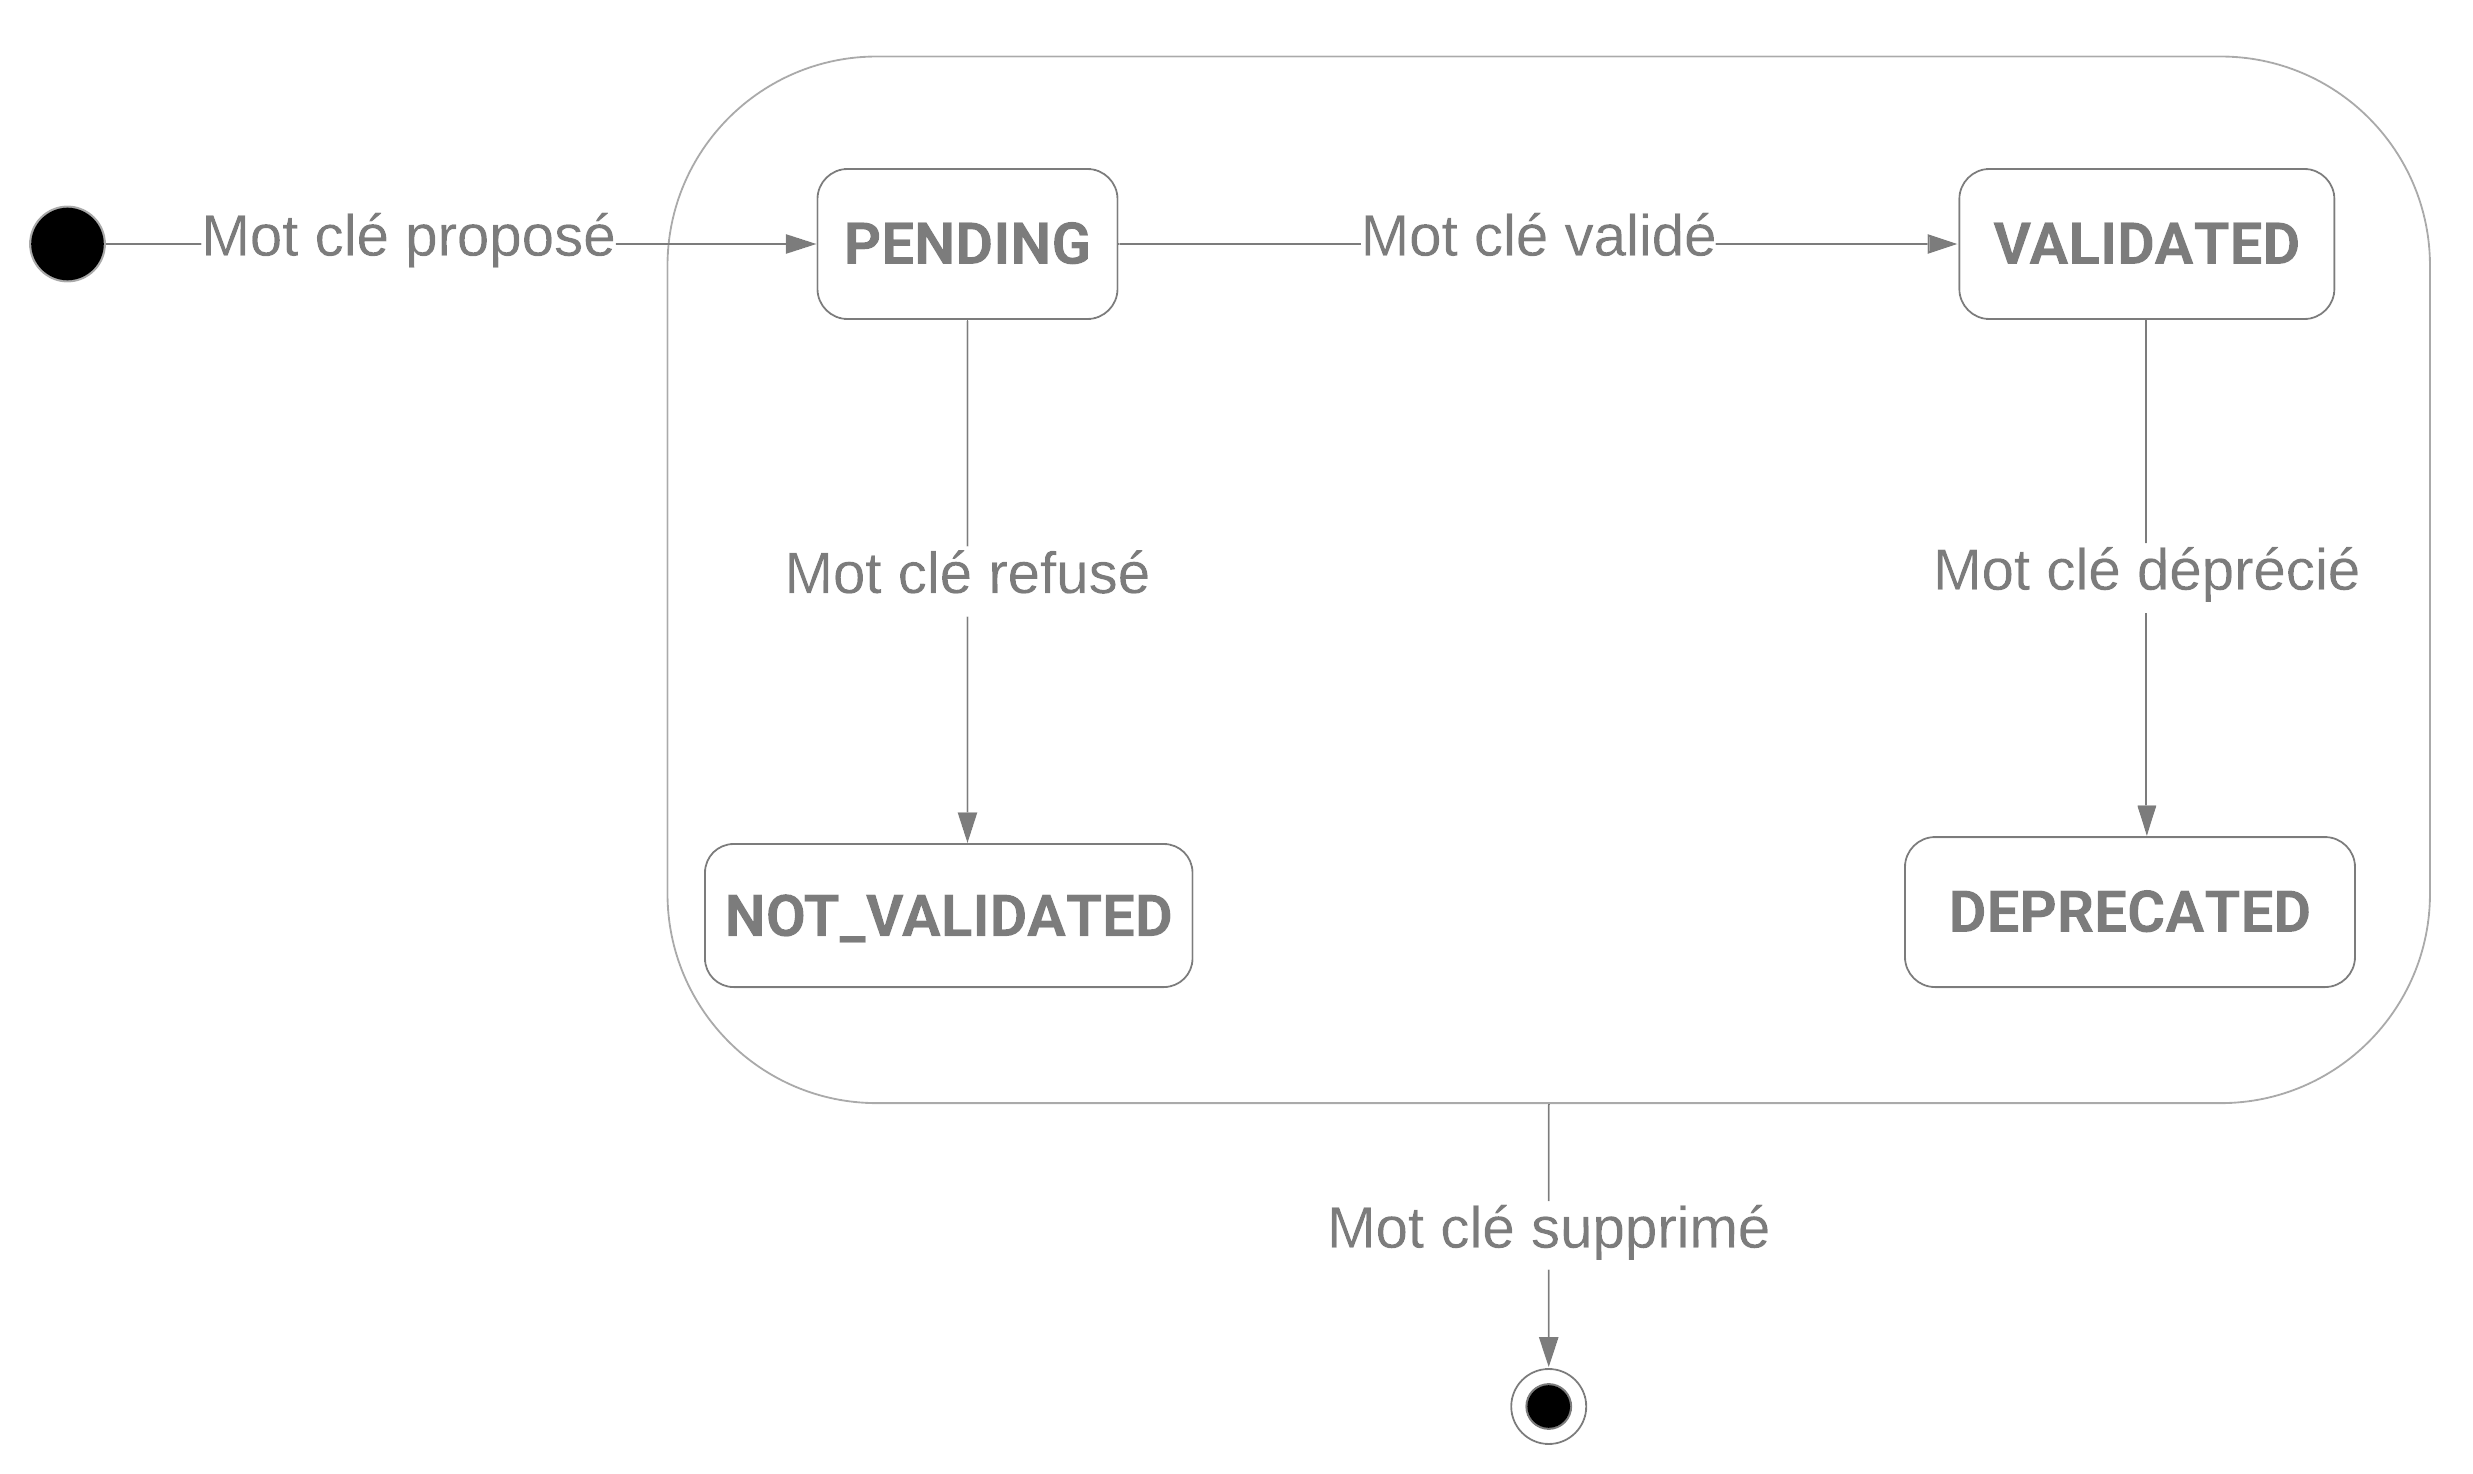
\includegraphics[width=\textwidth,height=\textheight,keepaspectratio]{images/StateTags.png}
    \centering
    \caption{Diagramme UML à états pour l'état d'un \gls{tag}}
    \label{pic:stateDiagramForTags}
\end{figure}

\subsection*{Maintenabilité aisée des données}

Lors de notre analyse, un besoin particulièrement criant s'est présenté à nous : sans être informaticien ou connaître les technologies réalisant le stockage de données, il faut disposer d'un moyen de lire/modifier ces données avec aisance. \\

Cela implique dès lors de proposer des opérations pour manipuler les différentes ressources de notre application ( \glspl{fiche}, \glspl{tag}, \glspl{tagCat}, etc... ). Pour compléter la panoplie, nous avons conçu un moyen d'importer / exporter les \glspl{fiche}, notamment pour répondre aux besoins d'archivage.

\pagebreak


\section{Analyse non-fonctionnelle}
% On explique ici ( design, ergonomie )
% Donner les critères d'ergonomie
% Pas forcément des tonnes de page : à priori 3-4 max devraient suffire

\subsection*{Securité}

La sécurité d'une application doit faire l'objet d'une attention non négligeable, particulièrement dans le contexte de notre époque mouvementée dans bien des domaines. Il est donc essentiel de se poser les bonnes questions ( par exemple en utilisant \Gls{QQOQCCP} ). Pour relever ce défi, une méthode possible est la \textbf{AAA}\footnote{Acronyme anglophone pour "\textbf{A}uthentication/\textbf{A}uthorization/\textbf{A}ccounting", que l'on peut traduire en français par "authentification/autorisation/traçabilité" }
consistant en 3 piliers : 

\begin{description}
    \item[Authentification :] Il s'agit du fait de prouver l'utilisateur que l'on prétend être. Une manière fréquemment utilisée sur de nombreux sites consiste en association d'un nom d'utilisateur et d'un mot de passe.
    \item[Autorisation :] Il s'agit du fait de vérifier quelles ressources accessibles et les opérations (par exemple les \Gls{crud}) permises sur celles-ci pour l'utilisateur authentifié.
    \item[Traçabilité :] Il s'agit du fait d'enregistrer tous les faits et gestes des utilisateurs authentifiés. Les informations ainsi collectées permettent principalement de prévenir/comprendre des problèmes. 
\end{description}

\subsection*{Maintenance et évolution}

\subsection*{Ergonomie}
TODO ( partie Alexandre )

\section {Contraintes}
% Expliquer les contraintes :
%    - Maintenabilité / Extensibilité  du code
%    - Gestion simple du système ( quand Mens disait que les admins ne devaient pas avoir à toucher à la DB pour faire x ou y truc )
%    - Interface orienté vers l'UX ( une jolie instruction UI VS UX
%    - etc...